\chapter{Surface-tension driven open microfluidic platform for hanging droplet culture}
\label{App:HangingDroplet}

\begin{figure}[ht] %DONE
\centering
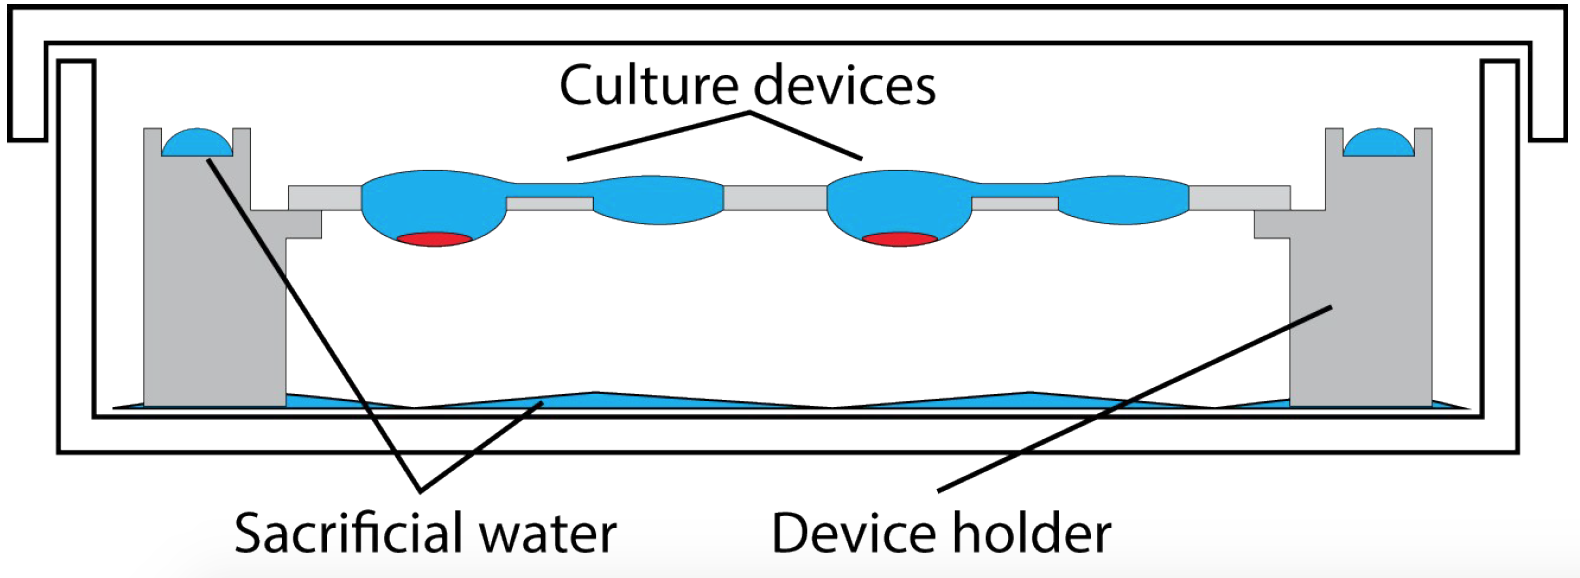
\includegraphics[width=4.5in]{/FigS1.png}
\caption{The device holder is placed in an OmniTray (Nunc) water is added to the bottom of the OmniTray and to the channel features of the device holder. The device is then placed into the device holder and filled with mediaand cells. The lid is placed on the OmniTray to ensure proper humidification of the device to prevent evaporation.}
\label{figure:FigS1}
\end{figure}

\begin{figure}[ht] %DONE
\centering
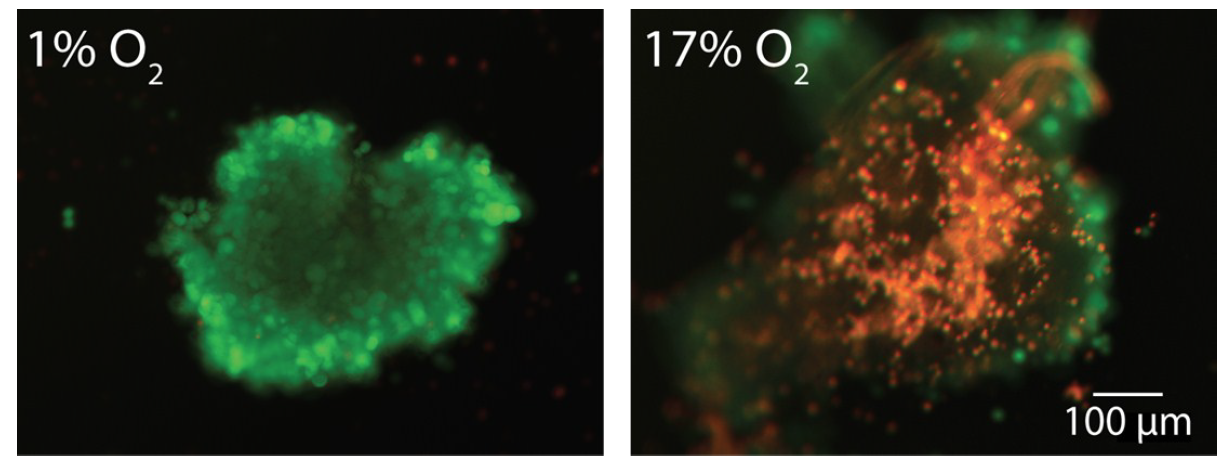
\includegraphics[width=4.5in]{/FigS2.png}
\caption{10,000 MDA-MB-231 cells were seeded into the culture well of the device and were cultured at either normoxic or hypoxic conditions for 48 hours before imaging. Live cells (green) were strained with calcein AM and dead cells were strained with ethidium homodimer (red). Spheroids were extracted from the device and transferred to a well plate for imaging. The hypoxic condition formed a markedly smaller spheroid with no low viability core, while the normoxic condition formed a spheroid with a low-viability, hypoxic core typical of what hasbeen previously observed}
\label{figure:FigS2}
\end{figure}

\begin{figure}[ht] %DONE
\centering
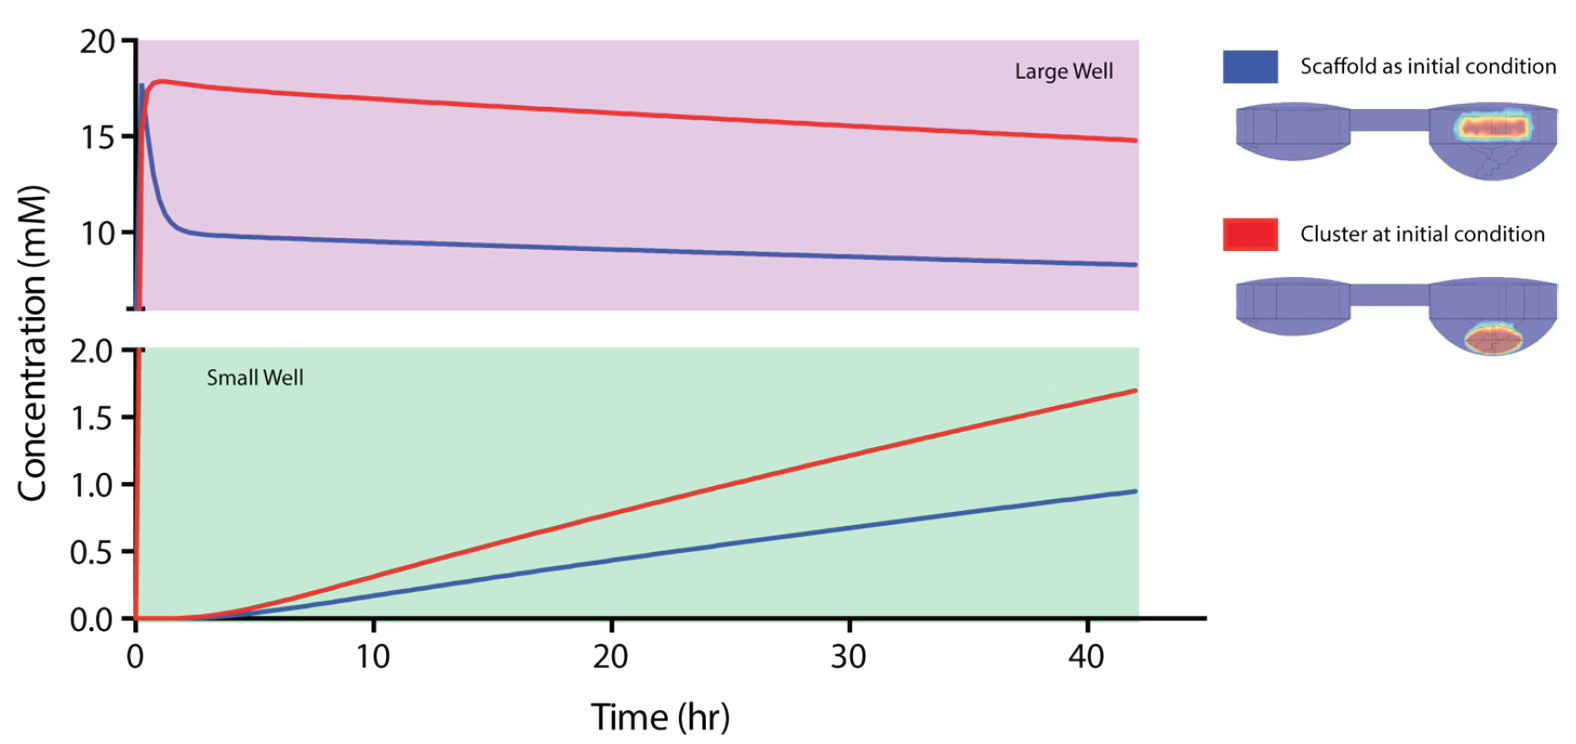
\includegraphics[width=4.5in]{/FigS3.png}
\caption{The average concentration in the bottom meniscus of each well following solute release in a modeled bone-like scaffold or cluster in the culture well.}
\label{figure:FigS3}
\end{figure}